\documentclass{beamer}
\usetheme{Madrid}
\usepackage{graphicx, hyperref, amsmath, animate}
\usecolortheme{beaver}
\graphicspath{{./plots/}}

\usepackage[backend=bibtex, style=numeric,sorting=none]{biblatex}
\addbibresource{ref.bib}
\renewcommand*{\bibfont}{\scriptsize}

\title{CS 725 - Foundations of Machine Learning}
\subtitle{Calorie Estimation of Food Items from Images}
\author{CV Maverics}
\institute[IITB]{Indian Institute of Technology Bombay}
\date{November 28, 2023}

\begin{document}
	% Title page frame
	\begin{frame}
		\titlepage
	\end{frame}
	
	% Outline frame
	\begin{frame}
		\frametitle{Outline}
		\tableofcontents
	\end{frame}
	
	% Section structure
	\section{Problem Statement}
	\begin{frame}{Problem Statement}
		\begin{columns}
			\column{0.5\textwidth}
			\begin{block}{Object Detection}
				\small Estimating calorie content from food images poses a significant challenge. In addressing this, the project strategically employs the You Only Look Once (YOLO) algorithm. This choice is pivotal in enhancing the accuracy of food item detection and classification.
			\end{block}
			\begin{block}{Calorie Estimation}
				\small Furthermore, the project incorporates the GrabCut algorithm to attain meticulous segmentation of food items in images. This precision is crucial for both volume estimation and, subsequently, accurate calorie estimation.
			\end{block}
			\column{0.45\textwidth}
			\begin{figure}
				\centering
				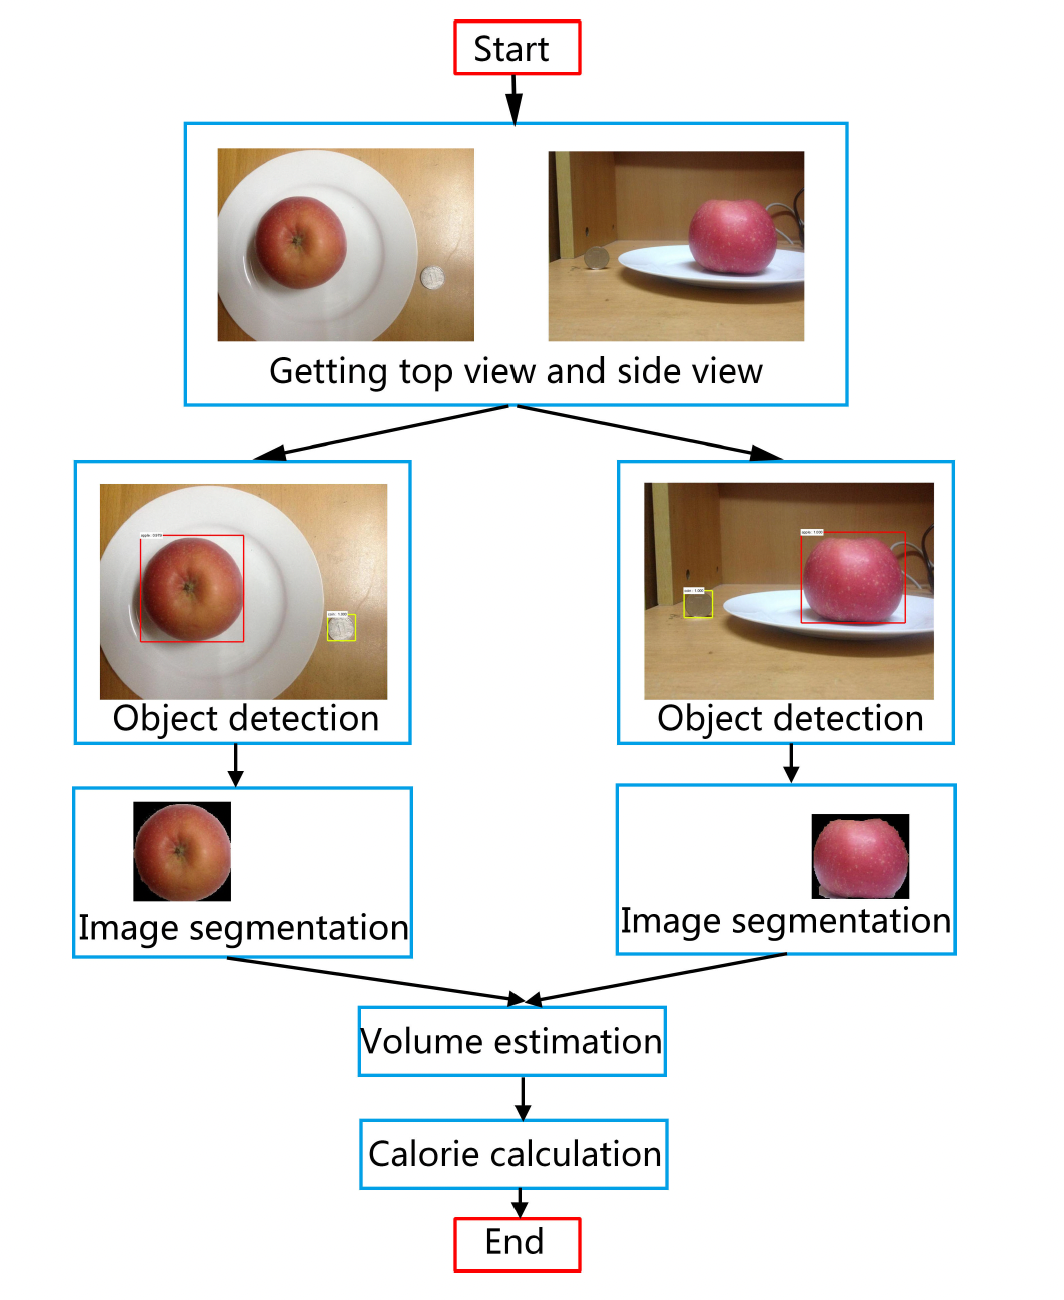
\includegraphics[scale=0.25]{roadmap.png}
				\caption{Calorie estimation of food items from images\cite{liang}}
			\end{figure}
		\end{columns}
	\end{frame}
	
	\section{Challenges Addressed}
	\begin{frame}{Challenges Addressed}\footnotesize
		\begin{block}{}
			\begin{description}
				\item[Dataset Acquisition:] Obtain and familiarize with the ECUST dataset. Understand the dataset's nuances, including its characteristics and potential challenges.
				\item[Data Preprocessing:] Prepare the dataset for model training. Resize images, normalize pixel values, and organize annotations. Ensure the dataset is well-structured and ready for training.\pause
				\item[Object Detection with YOLO:] Implement an effective object detection model. Deploy YOLO for food items detection and classification. Achieve accurate identification of food items in images.
				\item[Volume Estimation with GrabCut:] Accurately estimate the volume of segmented food items. Apply GrabCut algorithm for precise contour delineation. Obtain reliable volume information for further analysis.\pause
				\item[Calorie Content Estimation:]  Derive calorie content from volume and density values. Utilize obtained volume information to estimate the calorie content of each food item. Provide accurate assessments of the nutritional content.
				\item[Validation and Evaluation:] Assess the model's performance comprehensively. Include metrics such as mean absolute error. Ensure the model's effectiveness in calorie estimation.			
			\end{description}
		\end{block}
	\end{frame}
	
	\section{Outline of Method}
	\begin{frame}{Outline of Method}
		\begin{block}{Object Detection}\scriptsize
			\begin{itemize}
				\item The users capture top and side views of their food, including a One Yuan coin in each picture.
				\item The YOLO algorithm\cite{yolo} is employed for recognizing and outlining food types with precise bounding boxes.
			\end{itemize}
		\end{block}\pause
		\begin{block}{Image Segmentation}\scriptsize
			\begin{itemize}
				\item For image segmentation, each bounding box would be broken down into individual parts before volume estimation.
				\item The GrabCut algorithm\cite{grabcut} is utilized for image processing to obtain a precise outline of each food item. \item We then obtain segmented food images with background pixels replaced by zeros, focusing solely on foreground pixels.
			\end{itemize}
		\end{block}\pause
		\begin{block}{Calorie Estimation}\scriptsize
			\begin{itemize}
				\item Users provide images from both side and top views, including a One Yuan coin for scale.
				\item We then apply different formulas to estimate the volume of each food item.
				\item Using related calorie tables, we determine the calorie content of each food item.
			\end{itemize}
		\end{block}
	\end{frame}
	
	\begin{frame}{Outline of Method}
		\begin{block}{Volume Calculation}\tiny
			To estimate the volume\cite{vol}, we calculate the scale factors ($\alpha_S$ and $\alpha_T$) based on calibration object --- One Yuan coin.
			\begin{equation}
				\alpha_S = \frac{2.5}{(W_S + H_S)/2}; \quad
				\alpha_T = \frac{2.5}{(W_T + H_T)/2}
			\end{equation}
			Where $W_S, W_T$ and $H_S, H_T$ are the width and height of bounding box of coin in side and top view.
			\begin{equation}\label{E:vol}
				volume = 
				\begin{cases}
					\beta \cdot \frac{\pi}{4} \cdot \alpha_S^3 \cdot \sum_{k=1}^{H_S} (L^k_S)^2, &\text{if shape is ellipsoid} \\
					\beta \cdot  s_T \cdot \alpha_T^2 \cdot H_S \cdot \alpha_S, &\text{if shape is column} \\
					\beta \cdot  s_T \cdot \alpha_T^2 \cdot \alpha_S \cdot \sum_{k=1}^{H_S} \left(L^k_S/L_S^{max}\right)^2, &\text{if shape is irregular} 
				\end{cases}
			\end{equation}
			Where $L^k_S$ is the number of foreground pixels in side view of row $k$ ($k \in 1, 2, 3, \dots , H_S$). $L^{max}_S = \max_{k} L^k$. $\beta$ is a compensation factor (default value = 1.0).  $s_T$ is the surface area of the top view.
		\end{block}\pause
		\begin{block}{Evaluation Metric}\tiny
			We use mean absolute error as the evaluation metric for the volume estimation of each of the food item class.
			\begin{equation}
				MAE = \sum_{k=1}^{N} \frac{|v_{true}^k-v_{pred}^k|}{v_{true}^k}\times 100 \%
			\end{equation}
		\end{block}
	\end{frame}
	
	\section{Experiment Details and Main Results}
	\begin{frame}{Experiment Details and Main Results}
		\begin{block}{Dataset Processing}\scriptsize
			\begin{itemize}
				\item Utilized ECUST dataset with 19 diverse food types, each having top and side views.
				\item This dataset is a collection of 2978 images, each meticulously annotated and supplemented with necessary food metrics i.e. volume, density, calorie content etc.
				\item The images were calibrated images using a One Yuan coin (25 mm diameter) for accurate measurements.
				\item ECUST dataset considered important factors that affect the accuracy of estimation results: camera, lighting, shooting angle, displacement, calibration object, food type.
			\end{itemize}
		\end{block}\pause
		\begin{block}{Object Detection Setup}
			\begin{itemize}\scriptsize
				\item The food and fruit images are divided into train and test sets. We used 80-20 ordered split for training and testing set. 
				\item After YOLO version 8 is well trained, we use those pairs of test images which YOLO correctly recognizes to estimate volumes. In other words, those images YOLO cannot identity or misidentify in test sets will be discarded.
				\item We use mean absolute error to evaluate volume estimation results.
			\end{itemize}
		\end{block}
	\end{frame}
	
	\begin{frame}{Experiment Details and Main Results}
		\begin{block}{Volume Estimation Results}\scriptsize
			\begin{itemize}
				\item Volume estimation results are shown in the below Figure. For most types of food in our experiment, the estimation volume are closer to reference volume.
				\item The mean error between estimation volume and true volume does not exceed 20\% except banana, grape, mooncake. For some food types such as orange,our estimation result is close enough to the true value.
			\end{itemize}
			\begin{figure}
				\centering
				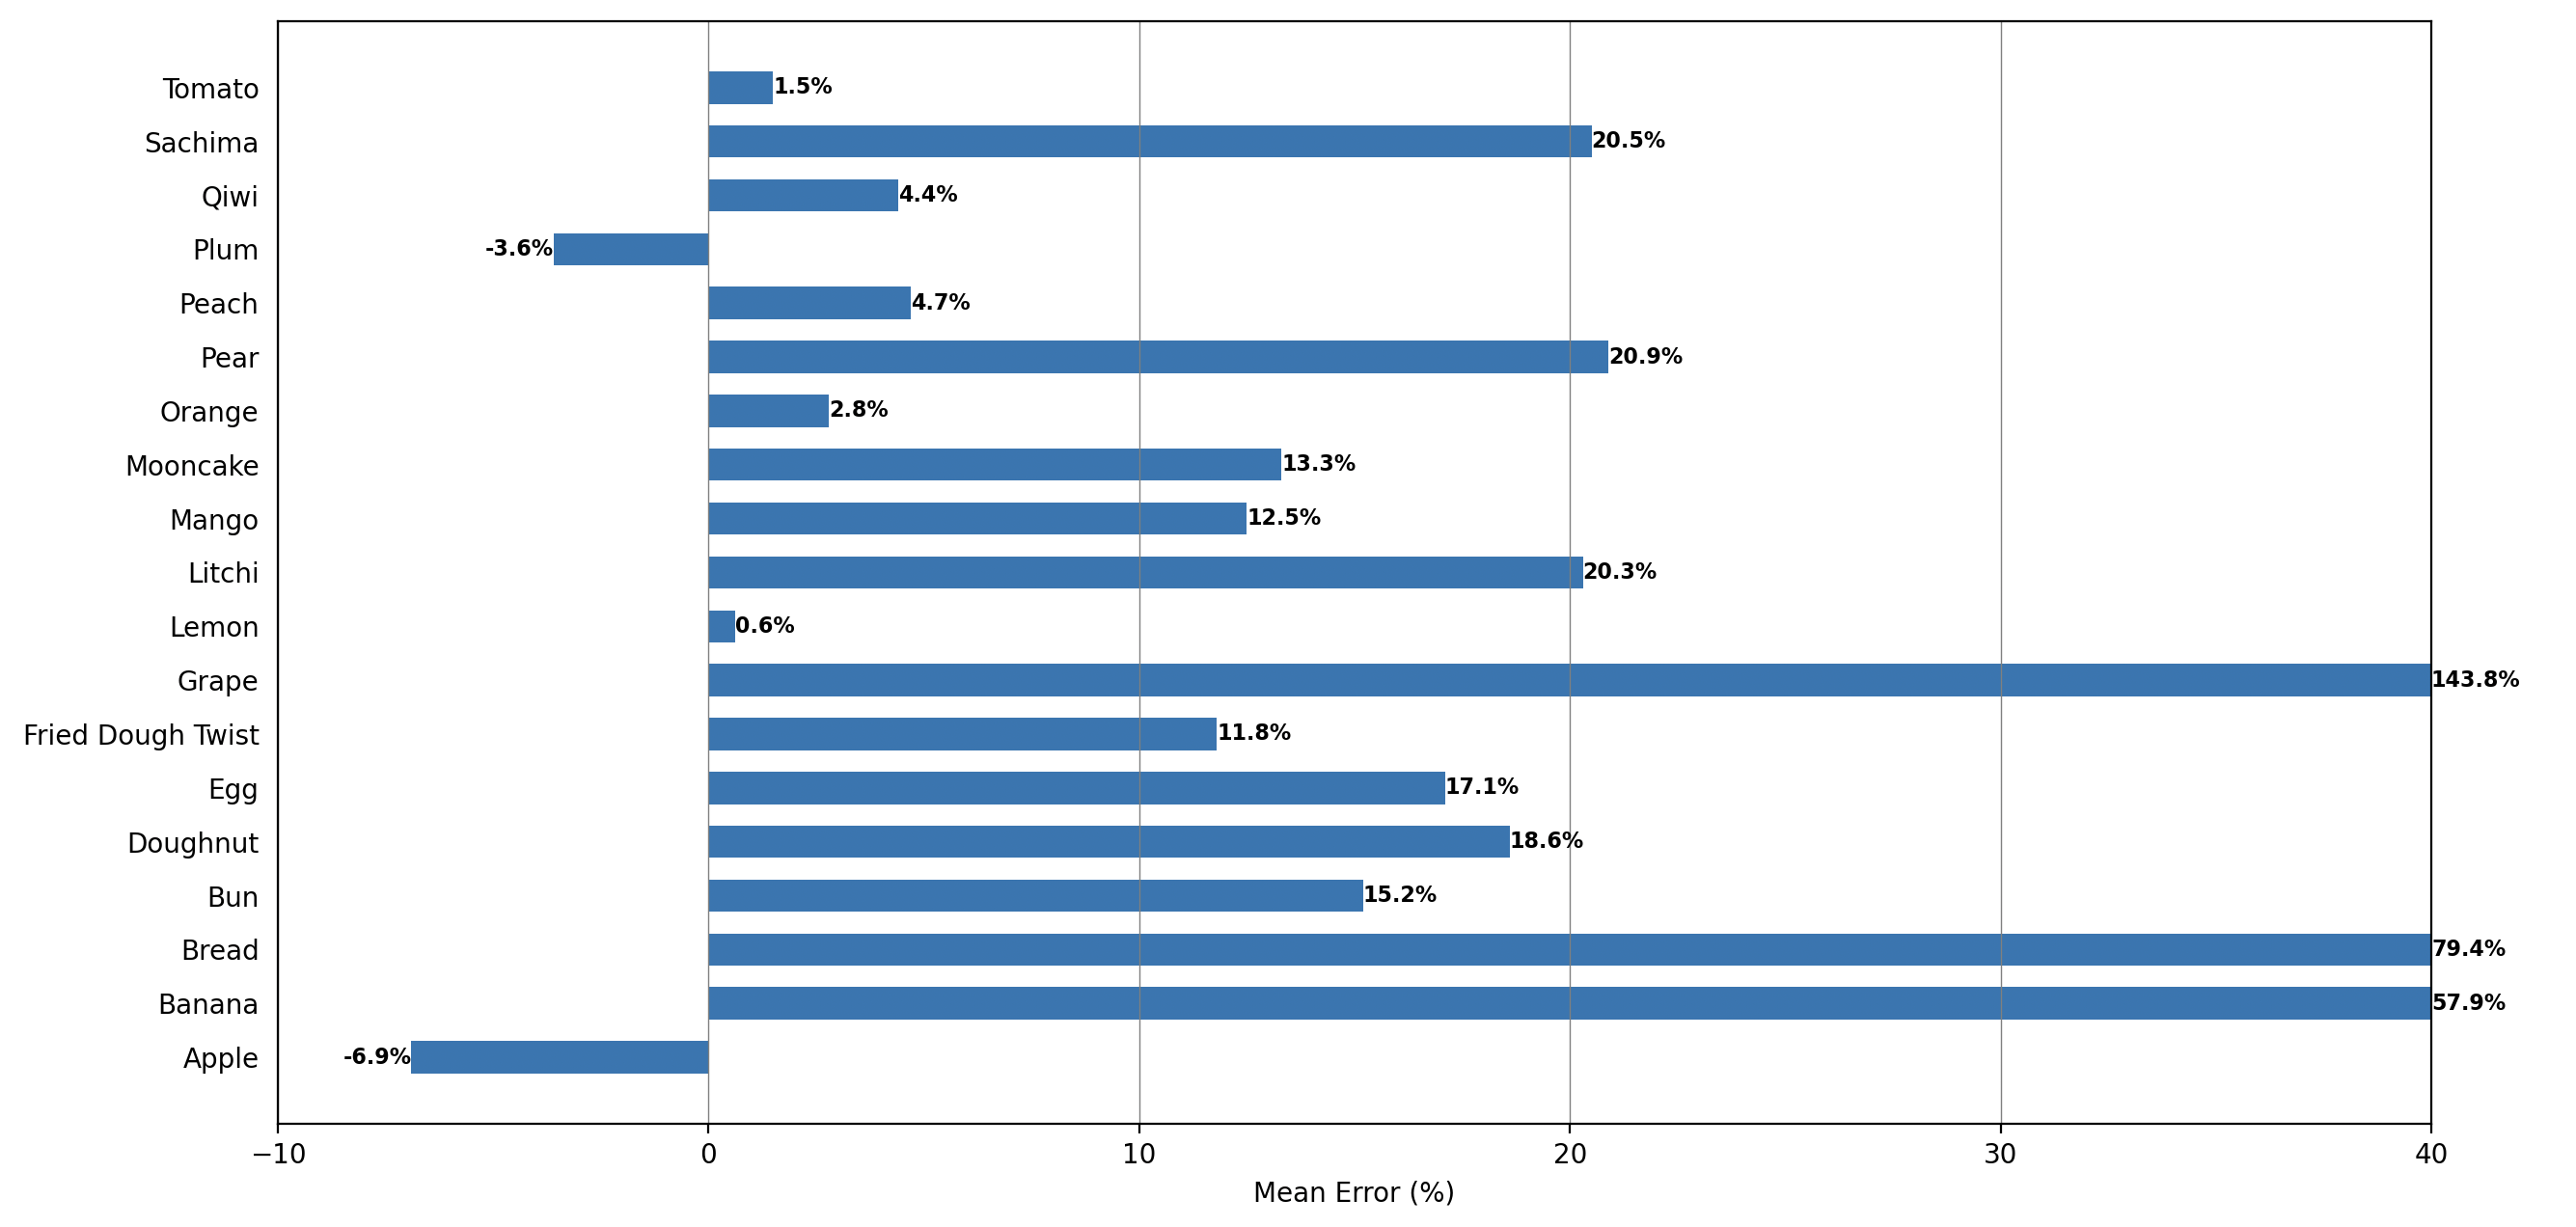
\includegraphics[scale=0.25]{vol_est.png}
				\caption{\scriptsize Volume estimation results of food items from images}
			\end{figure}
		\end{block}
	\end{frame}
	
	\section{Related Work}
	\begin{frame}{Related Work}
		\begin{block}{Previous Studies}\scriptsize
			\begin{itemize}
				\item Surveyed existing literature related to calorie estimation from food images.
				\item Identified key studies addressing challenges in object detection, volume estimation, and calorie assessment.
			\end{itemize}
		\end{block}
		\begin{block}{Object Detection Approaches}\scriptsize
			\begin{itemize}
				\item Explored methodologies in the literature for accurate detection and classification of food items.
				\item Noteworthy studies include \href{https://proceedings.neurips.cc/paper_files/paper/2015/file/14bfa6bb14875e45bba028a21ed38046-Paper.pdf}{Ren et al.} and \href{https://ieeexplore.ieee.org/stamp/stamp.jsp?arnumber=8978787}{Shang et al.}
			\end{itemize}
		\end{block}
		\begin{block}{Volume Estimation Techniques}\scriptsize
				\begin{itemize}
				\item Reviewed literature on precise volume estimation for food items in image analysis.
				\item Notable works include \href{https://arxiv.org/abs/1703.06870}{Girshik et al.} using Mask RCNN.
			\end{itemize}
		\end{block}
	\end{frame}
	
	\section{Conclusion}
	\begin{frame}{Conclusion}
		\begin{block}{}
			\begin{itemize}
				\item Successfully addressed the challenge of estimating calorie content from food images.
				\item Implemented a robust methodology utilizing YOLO for object detection and GrabCut for image segmentation.
				\item Leveraged the ECUST dataset with 2978 annotated images, overcoming challenges in dietary assessment.\pause
				\item Achieved key milestones in dataset utilization, preprocessing, object detection, volume estimation, and calorie content estimation.
				\item Validated and evaluated the model's performance, demonstrating effectiveness in accurate food item identification and calorie estimation.
			\end{itemize}
		\end{block}
	\end{frame}
	
	\section{Individual Contributions}
	\begin{frame}{Individual Contributions}
		\begin{block}{Team Members}\scriptsize
			\begin{description}
				\item [23M2157] Soumen Kumar Mondal
				\item [23M2162] Shubhranil B
				\item [23M2154] Siddhant Dnyanesh Gole
				\item [23M2156] Vaibhav Rathore
				\item [23M2158] Akash Pal
			\end{description}
		\end{block}
		\begin{block}{Contributions}\scriptsize
			\begin{description}
				\item [Soumen] Led the dataset acquisition and preprocessing efforts. Implemented and fine-tuned the YOLO model for efficient object detection. Handled documentation, code-base, report and presentation.
				\item [Vaibhav, Shubhranil] Applied expertise in image segmentation, incorporating the GrabCut algorithm. Contributed to the preparation of report.
				\item [Sidhhant, Akash] Contributed to the development of the calorie estimation workflow and validation processes. 
			\end{description}
		\end{block}
	\end{frame}
	
	\section{References}
	\begin{frame}{References}
		\begin{block}{Codebase}\scriptsize
			\begin{description}
				\item [Project Repo] All the works of the team can be found in this \textcolor{red}{ \href{https://github.com/soumenkm/CS725-FML-Project}{GitHub link}}.
				\item [Dataset Repo] The dataset can be found in this \textcolor{red}{ \href{https://github.com/Liang-yc/ECUSTFD-resized-}{GitHub link}}.
				\item [Volume Repo] This \textcolor{red}{ \href{https://github.com/Liang-yc/CalorieEstimation/blob/master/faster_rcnn-master/grabcut_mex.cpp}{GitHub link}} provided by Liang et al.\cite{liang} was referred to calculate the volume.
				\item [External Repo] The following libraries are used for the implementation of different algorithms --- \textcolor{red} { \href{https://docs.ultralytics.com/modes/train/}{Ultralytics}, \href{https://docs.opencv.org/3.4/d8/d83/tutorial_py_grabcut.html}{OpenCV}}
			\end{description}
		\end{block}
		\begin{block}{External Papers}\scriptsize
			\printbibliography
		\end{block}
	\end{frame}

\end{document}